\documentclass{article}

% Packages
\usepackage[utf8]{inputenc}
\usepackage{hyperref}
\usepackage{verbatim}
\usepackage{fancyvrb,newverbs,xcolor}
\usepackage{verbdef}
\usepackage[T1]{fontenc}
\usepackage{graphicx}
\usepackage{amsmath}
\usepackage{float}

\setlength{\parskip}{1em}
\verbdef{\vtext}{verb text}
\hypersetup{colorlinks=true}
\definecolor{cverbbg}{gray}{0.93}
\graphicspath{ {./img/} }

\newenvironment{lcverbatim}
 {\SaveVerbatim{cverb}}
 {\endSaveVerbatim
  \flushleft\fboxrule=0pt\fboxsep=.1em
  \colorbox{cverbbg}{%
    \makebox[\dimexpr\linewidth-2\fboxsep][l]{\BUseVerbatim{cverb}}%
  }
  \endflushleft
}

\newcommand{\inlverb}[1]{\colorbox{cverbbg}{\texttt{#1}}}

\renewcommand{\familydefault}{\sfdefault}

\title{Introducing Ranorex GUI testing within D-HYDRO}
\author{Prisca van der Sluis, Maarten Klapwijk}
\date{January 2022}

\begin{document}

\maketitle

\section{Introduction}

\section{Git Repository}

The Ranorex solution is located within the \href{https://github.com/Deltares/D-HYDRO.git}{D-HYDRO frontend repository}, directly within the \inlverb{./ranorex} folder. This folder contains the file \inlverb{DHYDRO.rxsln}, the Ranorex solution that can be opened by Ranorex. 

\section{Setting up your local Ranorex Environment}

\subsection{Setting up the floating license}

\begin{figure}[H]
\centering
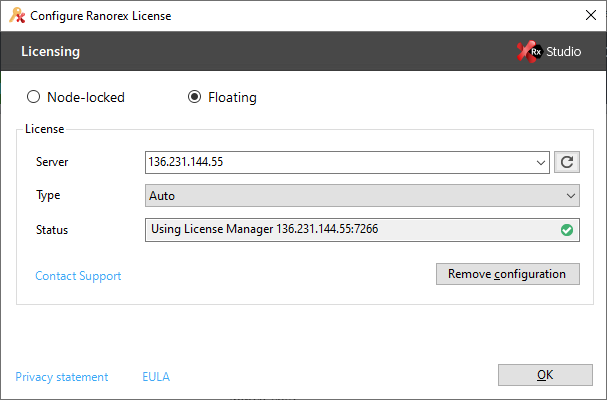
\includegraphics[scale=0.5]{license.png}
\label{fig:universe}
\end{figure}

A floating license is used for Ranorex. After installing Ranorex, you have to access the 'Ranorex Licensing' app.
For using a floating license, Server 136.231.144.55 has to be used. While remote working, note that you have to be connected to the Deltares VPN. Make sure you use the \textbf{same version} as the version that is used on the TeamCity agents.

\subsection{Setting up the test data}\label{sec:testdata}
We have decided to use a mapped network drive for handling test data. This has the benefits that we do not have to worry about correct file paths on different machines and the test data does not have to be checked out with each TeamCity build, the repository on the mapped drive is simply just updated.

For our Ranorex solution we use the \inlverb{R:} drive. To run the tests successfully on your machine, you have to set up a mapped network drive at \inlverb{R:} as well. You can do this manually, but the preferred way is to run the following script:
\begin{lcverbatim}
./ranorex/scripts/create_test_data.bat
\end{lcverbatim}

You can run the script by double clicking on it, which will use all the default parameters, or you can call the script from the command line providing the location where you want your test data to be. The script contains additional information and documentation. The default checkout location will be at:
\begin{lcverbatim}
.ranorex//test-data
\end{lcverbatim}

This location will be ignored by git.

You can also use the script to update the test data. 
The same script is used in the TeamCity environment to ensure that it has the same file structure as we have on our local machines.  


If you want to disconnect the mapping you can run the following in the command line:
\begin{lcverbatim}
net use R: /delete /y
\end{lcverbatim}

We decided on the following file structure for the test data:
\begin{lcverbatim}
<ROOT>
|---input
|   |---D-Flow_Flexible_Mesh
|   |   |---courses
|   |   |---tutorials
|   |---D-Morphology
|   |   |---courses
|   |   |---tutorials
|   |---D-Real_Time_Control
|   |   |---courses
|   |   |---tutorials
|   |---D-Water_Quality
|   |   |---courses
|   |   |---tutorials
|   |---D-Waves
|       |---courses
|       |---tutorials
|---output
|   |---D-Flow_Flexible_Mesh
|   |   |---courses
|   |   |---tutorials
|   |---D-Morphology
|   |   |---courses
|   |   |---tutorials
|   |---D-Real_Time_Control
|   |   |---courses
|   |   |---tutorials
|   |---D-Water_Quality
|   |   |---courses
|   |   |---tutorials
|   |---D-Waves
|       |---courses
|       |---tutorials
\end{lcverbatim}

The above illustration also contains an output folder, which will be created only when running the tests. 

\subsection{Location D-HYDRO executable}
The application executable is expected to be at the following location:
\begin{lcverbatim}
./bin/Release/DeltaShell/DeltaShell.Gui.exe
\end{lcverbatim}

so you have to build D-HYDRO in Release mode beforehand or copy the data you want to test to this location. There is a script at the following location:

\begin{lcverbatim}
./ranorex/scripts/build_d-hydro.bat
\end{lcverbatim}

When double-clicking on the file, the D-HYDRO solution will be automatically build in Release mode, without having to open Visual Studio for example.




\subsection{Setting up Report-to-pdf}
\label{sec:report_to_pdf}
The output report of a Ranorex run will be automatically converted to a pdf. To enable this, the \textit{Ranorex ReportToPDF} tool needs to be installed. In the project tree, right-click on the \textit{Solution DHYDRO}, \textit{Manage packages}, search for \textit{Ranorex ReportToPDF}, and click on \textit{add}.

Usually the tool also needs to be enabled in the section \textit{Ranorex Automation Helpers}, within the same project tree.





\subsection{Test data}
\subsubsection{D-Flow FM tutorials}\label{sec:fm_tutorials}
The D-Flow FM tutorial tests simulate the steps from the basic D-Flow FM tutorials. The tutorials are described in the D-Flow FM user manuals (\href{https://repos.deltares.nl/repos/ds/trunk/doc/user_manuals/dflowfm}{source code}, \href{https://dpcbuild.deltares.nl/buildConfiguration/DsDoc_ManualsValdationFunctionalityDocuments_ManualsLatexPdfRelease?}{compiled PDF}).
The \href{https://repos.deltares.nl/repos/ds/trunk/doc/user_manuals_tutorial_data/Tutorial_D-Flow_FM}{tutorial test data} should locally be checked out at (see: \ref{sec:testdata}):

\begin{lcverbatim}
D:/input/D-Flow_Flexible_Mesh/tutorials
\end{lcverbatim}



The D-Flow FM tutorial tests are part of the D\_FlowFM\_Tutorials test suite: \inlverb{D\_FlowFM\_Tutorials.rxtst}.


\subsubsection{D-Waq environmental modeling course}\label{sec:dwaq_env_mod}
The D-Waq environmental modeling course tests simulate the steps from the D-Waq environmental modeling course. The tutorials are described in the Delft4D FM Environmental modeling course reader (\href{https://repos.deltares.nl/repos/ds/trunk/doc/course_academy/delft3dm_environmental_modelling/reader}{source code}, \href{https://dpcbuild.deltares.nl/buildConfiguration/DsDoc_ManualsValdationFunctionalityDocuments_ManualsLatexPdfRelease?}{compiled PDF}).
The \href{https://repos.deltares.nl/repos/ds/trunk/doc/course_academy/delft3dm_environmental_modelling/exercises/input}{dwaq test data} should locally be checked out.



\subsubsection{Set global parameters}\label{sec:global_parameters}
For the D-Waq cases the input and output directories must be set as global parameters (right-click on \textit{WAQ - Test Suite}, followed by \textit{global parameters}):
\begin{lcverbatim}
    R:/input/courses/Environmental_modelling
\end{lcverbatim}
\begin{lcverbatim}
    R:/output/courses/Environmental_modelling
\end{lcverbatim}


\subsection{Run Ranorex}
It is important to note that Ranorex should be ran with \textbf{Administrator rights}. Tests might fail otherwise.

\section{TeamCity Configuration}

A project 'Ranorex tests' has been added to the D-HYDRO frontend project and can be found \href{https://dpcbuild.deltares.nl/project/DHydroUserInterface_DHydro_AutomatedTests_RanorexTests?mode=builds}{here}. This will be the root project of any Ranorex test configurations. 

\subsection{TeamCity agents}

Currently, all agents can run Ranorex. The resolution of the agents differs from the standard resolution on our laptops (1920 x 1080), potentially leading to problems.   

\subsection{Configuration: Tutorials D-Flow FM}

The \href{https://dpcbuild.deltares.nl/buildConfiguration/DHydroUserInterface_DHydro_AutomatedTests_RanorexTests_TutorialsDFlowFm?mode=builds}{D-Flow FM tutorial build configuration} automatically runs the D-Flow FM tutorials, see Section \ref{sec:fm_tutorials}.

The build configuration is dependent on the \href{https://dpcbuild.deltares.nl/buildConfiguration/DHydroUserInterface_DHydro_BuildConfiguration?mode=builds}{central build configuration} of D-HYDRO. This configuration builds the D-HYDRO solution in Release mode and publishes the resulting bin folder as an artifact. This bin folder is then copied into our own checkout, so that we save time by not having to build the entire D-HYDRO solution. 

\subsubsection{Build steps}

The D-Flow FM tutorial build configuration consists of multiple build steps:

\begin{enumerate}

    \item \textbf{Get Git Hash --} 
    Truncates the hash of the build number to 7 characters.
    
    \item \textbf{Update test data --}
    Runs the create\_test\_data.bat script (see: \ref{sec:testdata}).
    
    \item \textbf{Remove logs --}
    Removes the DeltaShell logs from the AppData folder that may have been generated in previous runs. 
    
    \item \textbf{Remove bin folder --}
    Removes the bin folder of the Ranorex solution if it exists.
    
    \item \textbf{Create nuget.config --}
    Creates a NuGet.Config file containing the correct NuGet feeds and credentials to authenticate with.
    
    \item \textbf{Restore packages --}
    Restores the NuGet packages in the Ranorex solution.
    
    \item \textbf{Build Ranorex solution --}
    Builds the Ranorex solution through MSBuild in Debug mode.
    
    \item \textbf{Run tests --}
    Starts up the generated test executable with and runs the selected test suite. 
    
    \item \label{copy_output} \textbf{Copy output files --}
    Copies all output files that were generated during the tests (saving or exporting data) into the checkout directory so that they can be published as artifacts and removes the output folder and content from the \inlverb{R:} drive.
    
    \item \label{disconnect_drive} \textbf{Disconnect mapped network drive --}
    Disconnects the \inlverb{R:} drive from the mapped location.
    
\end{enumerate}

Steps \ref{copy_output} and \ref{disconnect_drive} are always executed even if previous steps fail. 

\subsubsection{Artifacts}

The artifacts are divided into a couple of zip files.

\begin{enumerate}


    \item \textbf{deltashell\_log\_[githash].zip --} 
    Contains the log files produced by DeltaShell in the AppData folder.
    
    \item \textbf{output\_[githash].zip --} 
    Contains the output files produced as part of the tutorial during the tests when saving a project or exporting a model for example.
    
    \item \textbf{ranorex\_bin\_[githash].zip --} 
    Contains the whole bin folder of the Ranorex solution, making it easier to reproduce or pinpoint problems faster. 
    
    \item \textbf{ranorex\_reports\_[githash].zip --} 
    Contains the reports generated by Ranorex. These reports contain the results of the test cases including videos and screen shots of the application. 

\end{enumerate}

The artifacts are always published, regardless of the outcome of the build steps. 

\section{Ranorex set-up}

\subsection{Solution hierarchy}
The modules in the solution are structured based on the location in the UI it acts upon. For example, there are some modules that interact with the map, ribbon or project tree, etc. There are also modules that wait for a particular event to happen or interact with file dialogs, and these are grouped in a folder as well.

\subsection{Shared variables}
There are some variables that need to be shared throughout a single test case. These variables are best to keep in a \textbf{static variable} that can be accessed at any time.
At the time of writing we have two such variables. Both of them are located in the \inlverb{Current} class.

\begin{enumerate}
    \item \inlverb{Current.OutputDirectory} --
    This variable is and should be set during the setup of each test case that has some kind of output files (saving, exporting). The module \inlverb{SetCurrentOutputDirectory} makes sure that the variable is set with the correct value. 
    
    If you look at the data binding to this module in any of the test cases you can see that only the name of the tutorial is bound, which is the relative path to the directory where the output of this test case will be placed. The module makes sure that \inlverb{OutputDirectory} is set with the absolute path.
    
    For example, if you bind the following value to the module variable:
    
\begin{lcverbatim}
tutorial05
\end{lcverbatim}

The module then sets the \inlverb{Current.OutputDirectory} with the following path:

\begin{lcverbatim}
R:\output\tutorial05
\end{lcverbatim}

This variable can be used after the module has run until the end of the test case.

    \item \inlverb{Current.MapTransformation} -- 
 This variable can be used to get the currently calibrated pixels to interact with the map. Section \ref{sec:pixelcoords} elaborates on this. This variable is set during the execution of the \inlverb{CalibrateMap} code module and can be used afterwards in subsequent steps.
\end{enumerate}

There are also some \textbf{constant variables}. Changing them will affect all test cases. For example, we have the following variables:

\begin{enumerate}
    \item \inlverb{FileConstant.MappedDrive} -- This variable is set to \inlverb{R:}. This is the only location where the location of the mapped drive is defined. All file paths in the test cases will be made absolute using this variable.
    \item \inlverb{FileConstant.OutputDirectoryName} -- This variable is set to \inlverb{output} and is only defined here. This is the root folder for all output generated by the tutorials. Within this folder, folders are created for each tutorial that generates output. 
\end{enumerate}

It is advised to use constant variables when it makes sense to do so. Make sure you would only have to update a value in one place if needed.

\subsection{Screen pixels vs. world coordinates}\label{sec:pixelcoords}
Most action spots we define in Ranorex are \href{https://www.ranorex.com/blog/the-action-spot/}{"Proportional"}. We want to click at the center of most UI elements, such as a button. Tests relying on specific pixels can become unstable and unreliable. However, with some actions we do want to click on a specific pixel inside an element. The location of a pixel we need in a test depends on various factors such as the resolution of the running machine and the layout settings of the window controls. 

Interacting with the map control in D-HYDRO requires such specific location input, instead of proportional location input. In the map, we actually want to act at a certain world coordinate. To make sure that the tests are machine independent, we have to \textbf{calibrate the map} before any map interaction. This way, we can find the correct pixel location for the coordinate we need. We achieve this by following these steps:

\begin{enumerate}
    \item \textbf{Click one pixel (\(p1\)) in the top-left corner of the map}
    \item \textbf{Read and parse the displayed map coordinates (\(c1\)) in the status bar}
    \item \textbf{Click one pixel (\(p2\)) in the bottom-right corner of the map}
    \item \textbf{Read and parse the displayed map coordinates (\(c2\)) in the status bar}
    \item \textbf{Calculate the transformation} -- Two operations need to be taken into account: translation and scaling. 
    The scales in the \(x\) and \(y\) directions are respectively calculated by: 
    \begin{equation}
        s_x = \frac{ x_{p1} - x_{p2} } { x_{c1} - x_{c2} }
    \end{equation}
    \begin{equation}
        s_y = \frac{ y_{p1} - y_{p2} } { y_{c1} - y_{c2} }
    \end{equation}
    And the translations are calculated by:
    \begin{equation}
        t_x = x_{p1} - s_x x_{c1}
    \end{equation}
    \begin{equation}
        t_y = y_{p1} - s_y y_{c1}
    \end{equation}
    
    This calibration is performed when the \inlverb{CalibrateMap} module is called.
\end{enumerate}   
    
After the calibration, we can now calculate the pixel locations \(x_p\) and \(y_p\) corresponding to a given coordinate \(c\):
\begin{equation}
x_p = t_x + s_x x_c
\end{equation}
\begin{equation}
y_p = t_y + s_y y_c
\end{equation}

The \inlverb{Transformation} class contains this calculation and can be used by passing the coordinate.

\end{document}
